% Created 2019-07-29 Mon 14:55
% Intended LaTeX compiler: pdflatex
\documentclass[11pt]{article}
\usepackage[utf8]{inputenc}
\usepackage[T1]{fontenc}
\usepackage{graphicx}
\usepackage{grffile}
\usepackage{longtable}
\usepackage{wrapfig}
\usepackage{rotating}
\usepackage[normalem]{ulem}
\usepackage{amsmath}
\usepackage{textcomp}
\usepackage{amssymb}
\usepackage{capt-of}
\usepackage{hyperref}
\author{Wong Ding Feng}
\date{\today}
\title{Functional Programming: Real World Performance, Nix and Warp Server}
\hypersetup{
 pdfauthor={Wong Ding Feng},
 pdftitle={Functional Programming: Real World Performance, Nix and Warp Server},
 pdfkeywords={},
 pdfsubject={},
 pdfcreator={Emacs 26.2 (Org mode 9.2.2)}, 
 pdflang={English}}
\begin{document}

\maketitle
\tableofcontents

\section{Who am I? Introduction to myself}
\label{sec:orga745014}
\begin{itemize}
\item Follow me on github!
\url{https://github.com/TomatoCream}
\item Linux user for 5 years now
\begin{itemize}
\item Ubuntu
\item Proxmox
\item ArchLinux
\item Centos (server management)
\end{itemize}
\end{itemize}
\subsection{My interests}
\label{sec:org021a70a}
\begin{itemize}
\item AI, ML
\item Functional programming and abstraction (what the hell is so good about this?)
\item Philosophy
\begin{itemize}
\item occam's razor
<peekture>
\end{itemize}
\end{itemize}
\subsection{For whom is this talk for?}
\label{sec:org89b1014}
\begin{itemize}
\item Linux users! Sorry windows users
\begin{itemize}
\item But not really (departs away from a unix way of doing things)
\end{itemize}
\item Show you what functional programming can do?
\begin{itemize}
\item purity?
\item referential transparency?
\end{itemize}
\item State management
\item DevOps
\item Images, Docker, VM, Clusters
\end{itemize}
\section{The big problem}
\label{sec:org4854334}
\begin{itemize}
\item Has anyone ever used some sort of package management system?
\end{itemize}
\subsection{Some modern day package management systems}
\label{sec:orga736166}
\begin{center}
\begin{tabular}{ll}
Package manager & Distributions\\
\hline
apt, apt-get & Debian, Ubuntu\\
rpm, yum & Redhat, Centos\\
pacman & ArchLinux\\
brew & MacOS\\
\end{tabular}
\end{center}
\subsection{What about sub ecosystems?}
\label{sec:org479c34c}
\begin{center}
\begin{tabular}{ll}
Package manager & ???\\
\hline
pip, virtualenv, pipenv & Python2,3(???)\\
npm, yarn & Nodejs\\
cabal, stack, hackage & Haskell :)\\
go? & go?\\
brew & MacOS\\
use-package, vim, fish, zsh & \ldots{}\\
\end{tabular}
\end{center}
\subsection{How to make a package manager?}
\label{sec:org1da1c09}
\begin{itemize}
\item What are the basic parts that we need?
\end{itemize}
\subsection{How to make a package manager?}
\label{sec:orgb389177}
\begin{center}
\begin{tabular}{ll}
build dependencies & What do I need to build the program?\\
runtime dependencies & What \texttt{.so} shared objects do I need?\\
configurations & What in \texttt{/etc/...} config files\\
\end{tabular}
\end{center}
\begin{itemize}
\item essentially think of it as a graph, whenever we upgrade or install a package,
we are mutating a node on this graph to point to something else.
\end{itemize}
\subsection{Problems with modern package management}
\label{sec:org21030c9}
\url{https://wiki.debian.org/DontBreakDebian\#Don.27t\_make\_a\_FrankenDebian}
\begin{center}
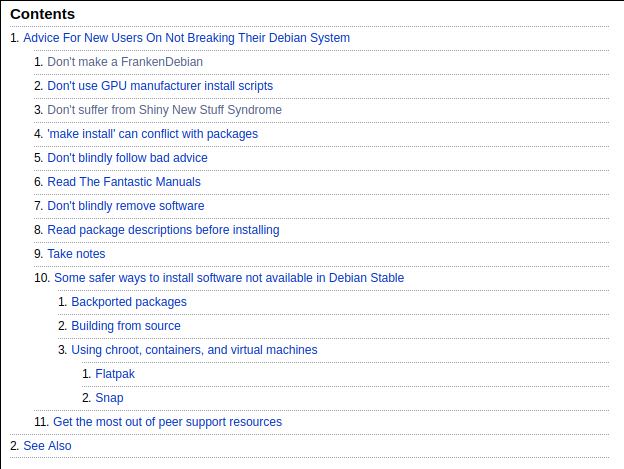
\includegraphics[width=.9\linewidth]{./images/screenshot-01.png}
\end{center}
\subsection{{\bfseries\sffamily TODO} Why imperative is bad? What is so imperative about installing packages?}
\label{sec:org6f4a87c}
referential transparency
\subsection{Are you familiar with \texttt{DEPENDENCY HELL}?}
\label{sec:orge9bba4c}
\begin{itemize}
\item \url{https://www.reddit.com/r/ProgrammerHumor/comments/75txp4/nodejs\_dependency\_hell\_visualized\_for\_the\_first/?utm\_source=share\&utm\_medium=web2x}
\item \url{https://github.com/vector-im/riot-web/network/dependencies}
\end{itemize}
\subsection{All types of "DEPENDENCY HELL"}
\label{sec:orgdfa5f70}
\url{https://miro.medium.com/max/984/0*7ezJOtYUkI5zyqWU.png}
\begin{itemize}
\item \{ DLL, dependency, npm, cabal \} hell, different names for the same demon
\item conflicting dependency
\begin{itemize}
\item shared components like library links \texttt{cuda.7.so} vs \texttt{cuda.6.so}
\end{itemize}
\item multiple version side by side and roll backs
\item possible solutions
\begin{itemize}
\item set of stable packages like \texttt{Debian} or \texttt{haskell stack snapshots}
\end{itemize}
\end{itemize}
\subsection{Not Atomic 01}
\label{sec:orgab758fb}
\begin{itemize}
\item kill upgrades half way
\begin{itemize}
\item packages left in a semi updated state
\item sometimes need to manually remove lock files
\end{itemize}
\end{itemize}
\begin{verbatim}
COMMAND   PID USER   FD   TYPE DEVICE SIZE/OFF   NODE NAME
dpkg    29329 root    3uW  REG    8,7        0 262367 /var/lib/dpkg/lock
\end{verbatim}
\subsection{Not Atomic 02}
\label{sec:org0dc6ed8}
\begin{itemize}
\item can be fixed but kinda troublesome.
\end{itemize}
\begin{center}
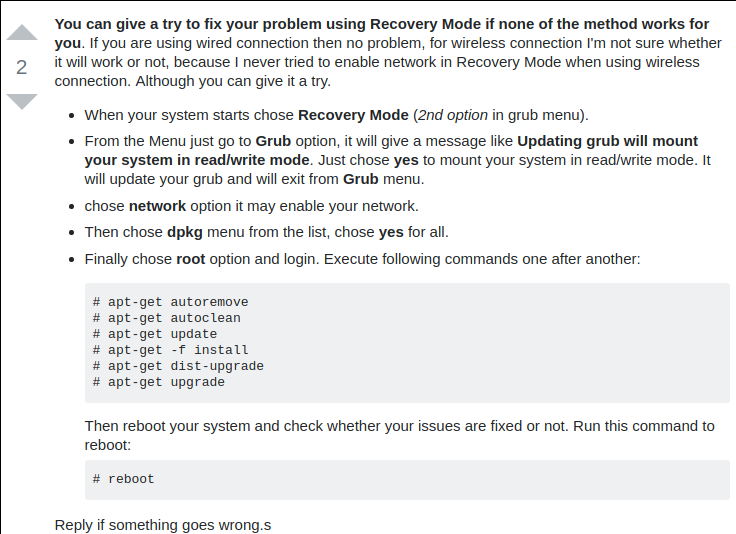
\includegraphics[width=.9\linewidth]{./images/screenshot-02.png}
\end{center}
\subsection{Whats bad about imperative summary?}
\label{sec:org48bd486}
\begin{itemize}
\item No referential transparency
\begin{itemize}
\item cannot point to older versions of the same thing
\end{itemize}
\item Dependency hell
\begin{itemize}
\item conflicting dependencies
\end{itemize}
\item Not atomic upgrades
\begin{itemize}
\item unknown state if break half way
\end{itemize}
\end{itemize}
These problems are really similar to the problems with imperative languages!
like \texttt{JAVA} and people have already made solutions for them like how \texttt{Haskell}
does. We could learn a thing or two from them.
\section{What it should/could/would have been?}
\label{sec:org919f056}
\begin{itemize}
\item Imagine now that we implemented all the things of a functional programming
language to create a functional package management system?
\item What can we do with this?
\end{itemize}
\subsection{GUIX vs Nix}
\label{sec:org7c83c1c}
\begin{itemize}
\item \begin{center}
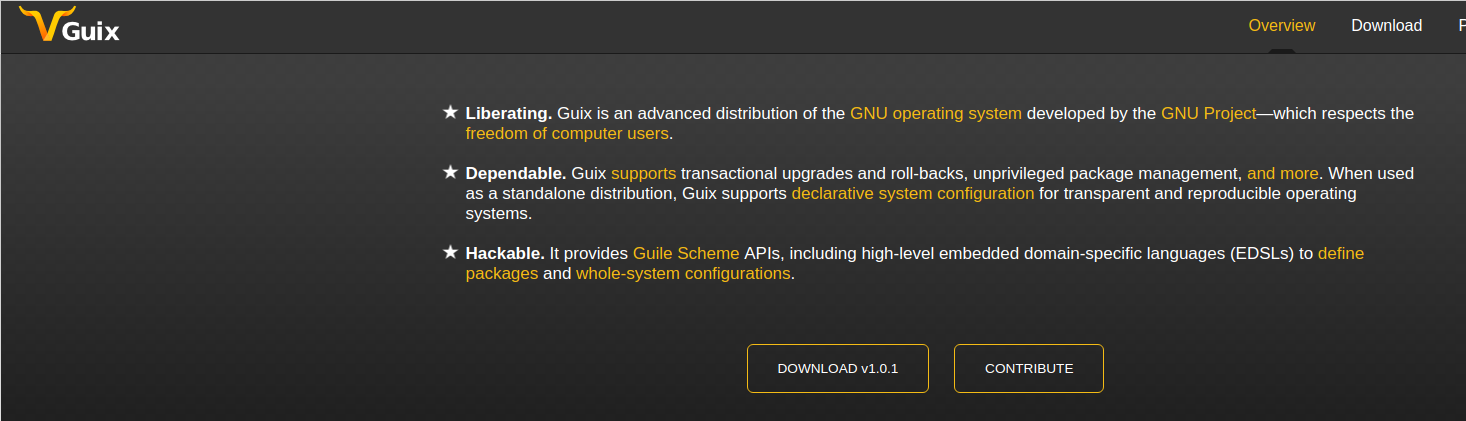
\includegraphics[width=.9\linewidth]{./images/screenshot-04.png}
\end{center}
\item \begin{center}
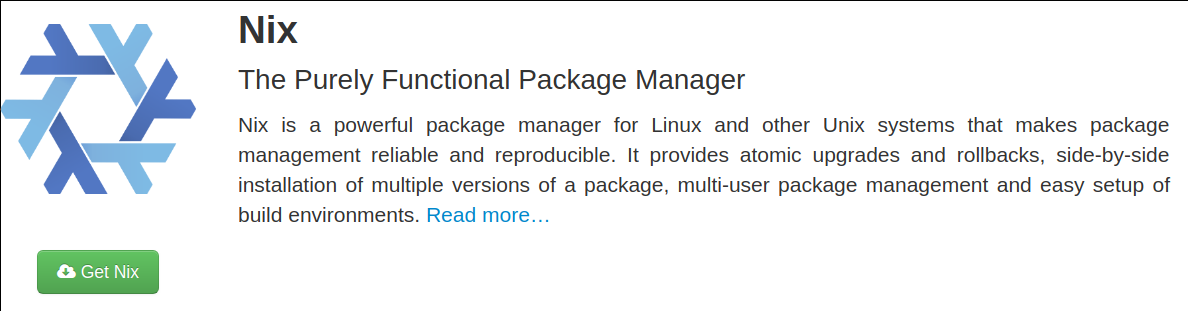
\includegraphics[width=.9\linewidth]{./images/screenshot-03.png}
\end{center}
\end{itemize}
\subsection{Introducing Nix Package Management}
\label{sec:org34d31ce}
\begin{itemize}
\item solves all of the problems above
\begin{itemize}
\item No referential transparency
\begin{itemize}
\item cannot point to older versions of the same thing
\end{itemize}
\item Dependency hell
\item Not atomic upgrades
\begin{itemize}
\item unknown state if break half way
\end{itemize}
\end{itemize}
\end{itemize}
\subsection{Main mechanism}
\label{sec:orga6ea085}
\begin{itemize}
\item referential transparency
\begin{itemize}
\item install everything in path \texttt{/nix/store/\{hash\}-name}
\item via \texttt{symlinking}
\end{itemize}
\end{itemize}
\subsection{What you get for free with this mechanism?}
\label{sec:orgb489144}
\begin{itemize}
\item no \texttt{sudo}
\item easy revert and roll back
\item 2 different version can run at the same time
\item same \textbf{development} environment as the \textbf{runtime} environment!
\begin{itemize}
\item nix-shell
\end{itemize}
\end{itemize}
\subsubsection{no \texttt{sudo}, where is my \texttt{sudo}?}
\label{sec:org87caf5b}
\begin{itemize}
\item linux was developed as a \texttt{time sharing} system
\item many users were expected to share a single computer.
\item thus to manage conflicts, a \texttt{super user}, \texttt{root} was required to
install and manage packages
\begin{verbatim}
nix-env -iA nixos.figlet
\end{verbatim}
\end{itemize}
\subsubsection{easy revert, rollback}
\label{sec:org2e708e6}
\begin{verbatim}
figlet "I am here!"
\end{verbatim}
\begin{verbatim}
nix-env --rollback
\end{verbatim}
\begin{verbatim}
figlet "are you still here?"
\end{verbatim}
\subsection{Going all the way, NixOS}
\label{sec:org5474470}
\begin{itemize}
\item whole system management via Nix
\begin{itemize}
\item Version controlled operating system
\item show OS reboot
\end{itemize}
\end{itemize}
\subsection{There are actually 2 players}
\label{sec:org744437c}
\end{document}
